\documentclass{beamer}
\usepackage{graphicx}
\usepackage{tikz}
\usetikzlibrary{shapes,arrows}
\usepackage{tikz}
\usetheme{default}
%\usecolortheme{seahorse}
\usepackage{default}

  \setbeamertemplate{footline}[page number]
\setbeamertemplate{navigation symbols}{}
\setbeamertemplate{frametitle}[default][center]
\setbeamerfont{frametitle}{shape=\scshape}

\usepackage{color}

\usepackage{media9}%
\newcommand{\includemovie}[3]{%
\includemedia[%
width=#1,height=#2,%
activate=pagevisible,%
deactivate=pageclose,%
addresource=#3,%
flashvars={%
src=#3 % same path as in addresource!
&autoPlay=true % default: false; if =true, automatically starts playback after activation (see option ?activation)?
&loop=true % if loop=true, media is played in a loop
&controlBarAutoHideTimeout=0 %  time span before auto-hide
}%
]{}{StrobeMediaPlayback.swf}}%


{\title{\textsc{Numerical Methods-Lecture 6: Other Methods}}
\author{Trevor Gallen}
\date{}

\begin{document}

\begin{frame}
\titlepage
\end{frame}

\begin{frame}
\frametitle[alignment=center]{Motivation}
\begin{itemize}
\item Newton's Method has flaws
\bigskip
\item Mostly, computing Jacobian or Hessian is hard, not always possible
\bigskip
\item Want to consider derivative-free alternatives
\end{itemize}
\end{frame}

\begin{frame}
\frametitle[alignment=center]{List}
\begin{itemize}
\item Bisection
\bigskip
\item Golden section search
\bigskip
\item Nelder-Mead Simplex
\bigskip
\item Conjugate Gradient Method
\bigskip
\item Evolutionary, Simulated Annealing
\bigskip
\end{itemize}
\end{frame}

\begin{frame}
\frametitle[alignment=center]{Bisection Method}
\begin{itemize}
\item The Bisection method is what you use naturally when looking for a zero.  \ \\
\bigskip
\item Univariate
\bigskip
\item Want to find a root between $a$ and $b$
\bigskip
\item Denote new values of $a$ and $b$ with $a'$ and $b'$.
\bigskip
\begin{enumerate}
\item Take two points, $a$ and $b$, where $f(a)<0<f(b)$.
\bigskip
\item Evaluate $f(\frac{a+b}{2})$ (Let $c=\frac{a+b}{2}$).
\bigskip
\item If $f(c)<0$, then $a'=c$.  If $f(c)>0$, then $b'=c$.
\bigskip
\item Repeat.
\end{enumerate}
\end{itemize}
\end{frame}

\foreach \x in {1,2,...,7}
{
\begin{frame}
\frametitle[alignment=center]{Bisection Method, Graphically}
\begin{figure}[htdb!]
\centering
\includegraphics[scale=0.8]{Bisection_\x.png}
\end{figure}
\end{frame}
}


\begin{frame}
\frametitle[alignment=center]{Golden Section Search}
\begin{itemize}
\item Golden Section Search is roughly what you use naturally when looking for a minimum.  \ \\
\item Univariate
\item Want to find a minimum $a$ and $b$
\item Denote new values of $a$ and $b$ with $a'$ and $b'$.
\begin{enumerate}
\item Take interval defined by $(a,b)$, $a<b$.
\item Evaluate $c=b-\phi(b-a)$, $d=a+\phi(b-a)$
\item If $f(c)>f(d)$, then $a'=c$, $b'=b$.   If $f(c)<f(d)$, $a'=a$, $b'=d$.
\item Repeat.
\end{enumerate}
\item Initial choice of three points: given $a$ and $c$, choose $b=1.618a$, golden ratio.
\item One can show that this ensures that no matter which point is best, $a$, $b$, $c$, $d$ always keep same relative distance: this avoids just using one interval all the time because we were too close to minimum with first point.
\end{itemize}
\end{frame}

\foreach \x in {1,2,...,4}
{
\begin{frame}
\frametitle[alignment=center]{Golden Section Search, Graphically}
\begin{figure}[htdb!]
\centering
\includegraphics[scale=0.8]{Golden_\x.png}
\end{figure}
\end{frame}
}

\begin{frame}
\frametitle[alignment=center]{Univariate Methods}
\begin{itemize}
\item Univariate methods have limited usefulness
\bigskip
\item Bisection frequently useful when you have bounds and a simple problem: negotiation weights problem, how much to work, etc.
\bigskip
\item Alternatively, Golden section search is more often used by taking multivariate problem, finding direction, then minimizing using Golden section search, repeating
\end{itemize}
\end{frame}


\begin{frame}
\frametitle[alignment=center]{Conjugate Gradient Method}
\begin{itemize}
\item Conjugate gradient doesn't require Jacobian, just gradient.
\bigskip
\item We're going to keep track of search direction $S_n$ (a vector)
\bigskip
\item For legibility, define steepest direction $\Delta X_n=-\nabla_xf(X_N)$
\bigskip
\item Start first search direction as steepest descent: $S_0=\Delta X_0$
\end{itemize}
\end{frame}


\begin{frame}
\frametitle[alignment=center]{Conjugate Gradient Method}
\begin{itemize}
\item Starting at $t=0$, with $S_0=-\nabla f(X_0)$
\begin{enumerate}
\item Calculate $\Delta X_t$ by taking gradient.
\item If $t>0$, update search direction: $S_{t}=\Delta X_t+\frac{\Delta X_t'\Delta X_t}{\Delta X_{t-1}'\Delta X_{t-1}} S_{t-1}$
\item Along the plane defined by $S_t$, find $\alpha^*$ to minimize $f$:
$$\arg\underset{\alpha}{\min}f(X_t+\alpha_t S_t) $$
\item Using $\alpha_t^*$, update $X_{t+1}$:
$$X_{t+1}= X_t+\alpha_t^* S_t$$ 
\item Repeat
\end{enumerate}
\end{itemize}
\end{frame}

\foreach \x in {1,2,...,41}
{
\begin{frame}
\frametitle[alignment=center]{Conjugate Gradient: Examples}
\includegraphics[scale=0.5]{Conjugate_Gradient_\x.png}
\end{frame}
}

\begin{frame}
\frametitle[alignment=center]{Derivative-Free Methods}
\begin{itemize}
\item Nelder-Mead Simplex 
\bigskip
\item Pattern search
\bigskip
\item Differential evolution/Genetic algorithms
\bigskip
\item Simulated Annealing
\end{itemize}
\end{frame}

\begin{frame}
\frametitle[alignment=center]{Nelder Mead}
\begin{itemize}
\item Nelder-Mead is fun, simple, fairly robust
\bigskip
\item Makes great intuitive sense
\bigskip
\item Easy for it to stop at local minima
\bigskip
\item Not as fast as derivative-based
\bigskip
\item Not as slow as differential evolution
\bigskip
\item If it starts out making sense, it rarely ends not making sense
\end{itemize}
\end{frame}

\begin{frame}
\frametitle[alignment=center]{Nelder Mead: the idea}
\begin{itemize}
\item You have an n-dimensional problem (for instance, 2-d)
\item Take n+1 verticies in those n dimensions  (for instance, 3 points)
\item Either improve the worst point using all other points or shrink the simplex
\begin{itemize}
\item ``Reflect" or ``flip" the worst point over the body of the simplex to look for a better point
\item If that worked okay, then stop
\item If that worked very well, move it even further (expansion)
\item If that improved things, use expanded point, otherwise, use reflected point.
\item If that didn't work well, then move point closer to body but don't flip
\item If this works, then use it
\item If this didn't work, shrink everyone's distance from the best point
\end{itemize}
\item Continue until near a minimum/maximum
\end{itemize}
\end{frame}

\foreach \x in {1,2,...,7}
{
\begin{frame}
\frametitle[alignment=center]{Nelder Mead: Step Examples}
\includegraphics[scale=0.5]{Nelder_Mead_\x.png}
\end{frame}
}

\begin{frame}
\frametitle[alignment=center]{Pattern Search}
\begin{itemize}
\item Pattern search is what you'd do if you didn't trust the terrain
\item Only thing that competes with steepest descent for most natural
\item Pick a stepsize
\item One at a time, perturb your point in only one direction by the stepsize
\item If things are improved, move there, sample more points
\item If not, shrink the step size
\item There are lots of variations on this theme
\begin{itemize}
\item Your basis vector doesn't have to be $x\pm\left[\begin{array}{c}d \\ 0\end{array}\right]$ and $x\pm\left[\begin{array}{c}0 \\ d\end{array}\right]$
\item It could be $x\pm\left[\begin{array}{c}d \\ 0.5d\end{array}\right]$ and $x\pm\left[\begin{array}{c}-0.5d \\ d\end{array}\right]$
\item Could choose random orthogonal vectors
\item Could immediately take improving step, or could search more, etc.
\end{itemize} 
\end{itemize}
\end{frame}

\begin{frame}
\frametitle[alignment=center]{Pattern Search: Example}
\begin{figure}
\centering
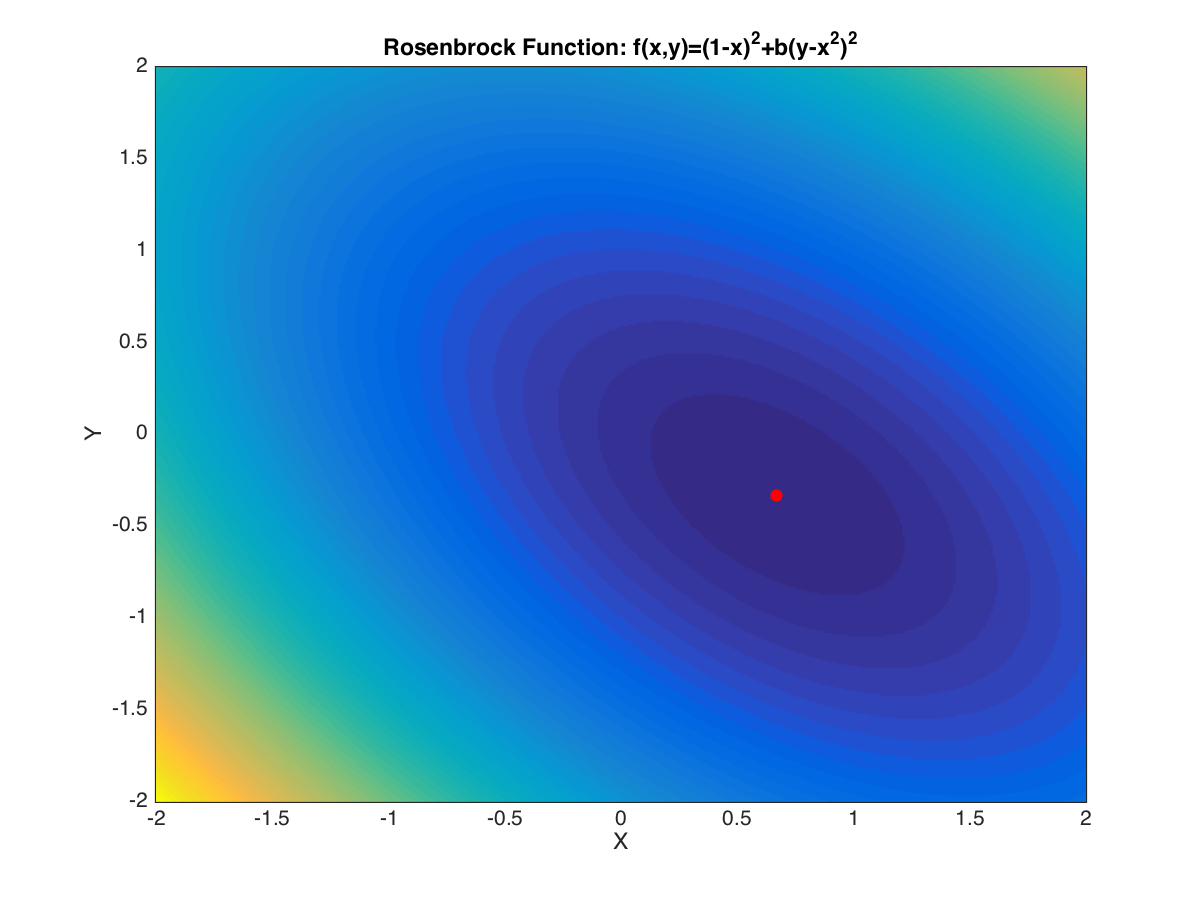
\includegraphics[scale=0.5]{PatternSearch_1.png}
\end{figure}
\end{frame}

\foreach \x in {3,4,...,15}
{
\begin{frame}
\frametitle[alignment=center]{Pattern Search: Example}
\includegraphics[scale=0.5]{PatternSearch_\x.png}
\end{frame}
}



\begin{frame}
\frametitle[alignment=center]{Pattern Search: Non-Cartesian Basis}
\begin{figure}
\centering
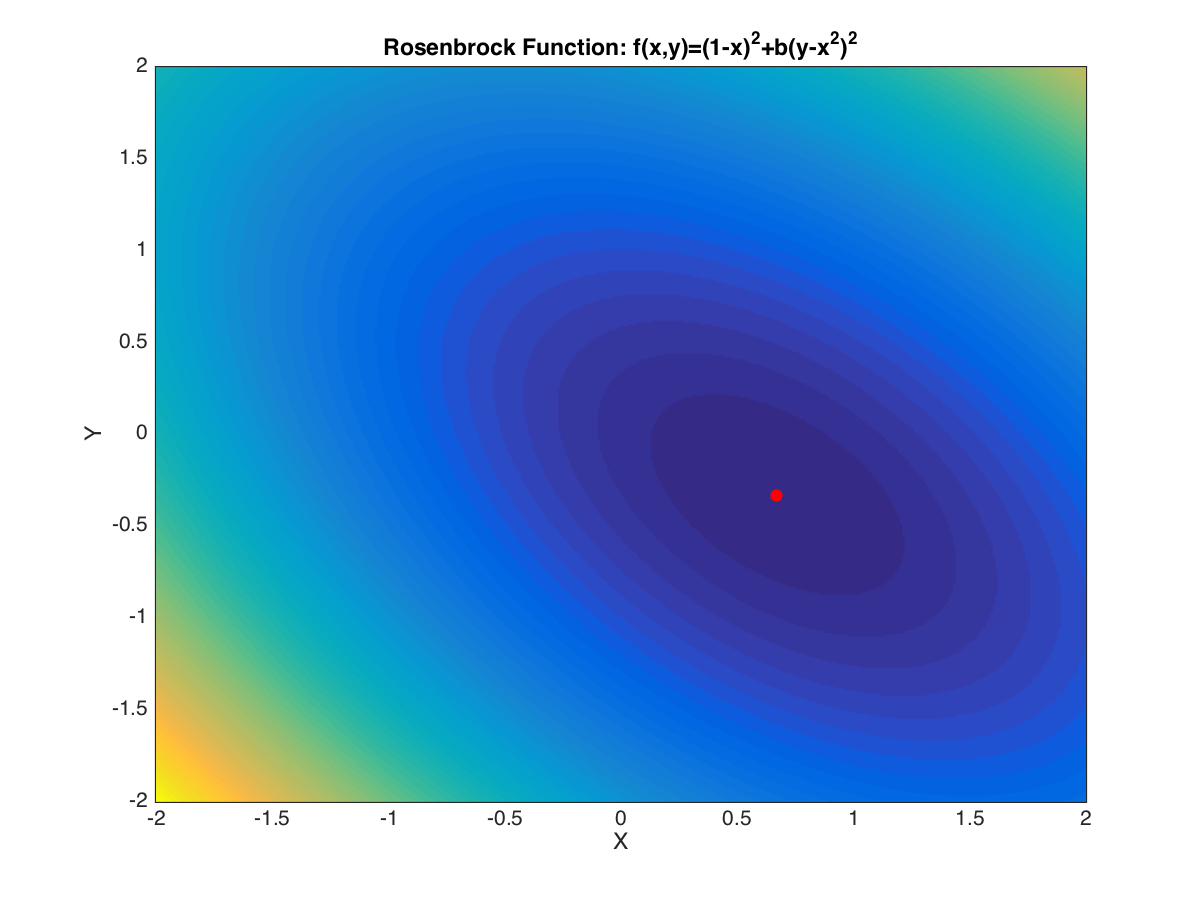
\includegraphics[scale=0.5]{PatternSearch_1.png}
\end{figure}
\end{frame}

\foreach \x in {3,4,...,15}
{
\begin{frame}
\frametitle[alignment=center]{Pattern-Search: Non-Cartesian Basis}
\includegraphics[scale=0.5]{PatternSearch_Ne_\x.png}
\end{frame}
}



\begin{frame}
\frametitle[alignment=center]{Pattern Search: Random Basis}
\begin{figure}
\centering
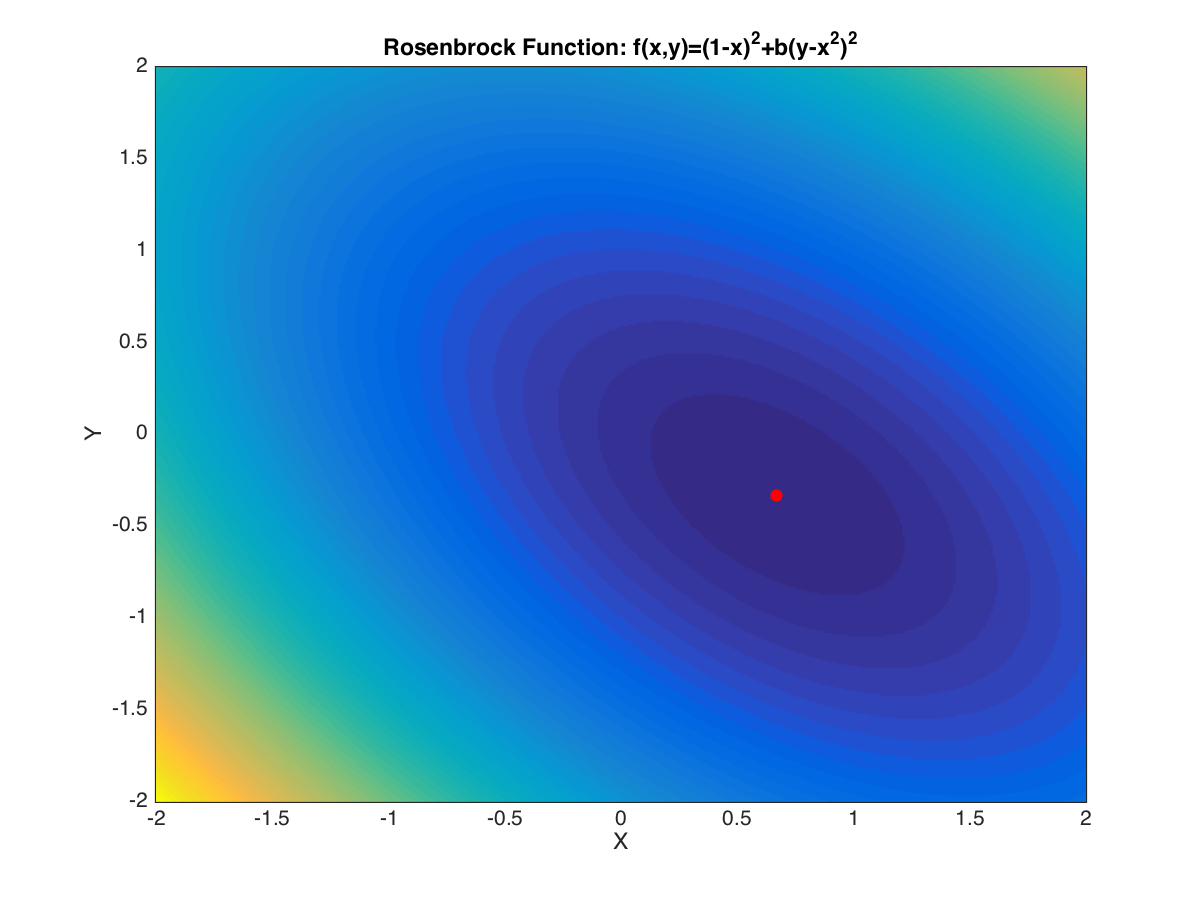
\includegraphics[scale=0.5]{PatternSearch_1.png}
\end{figure}
\end{frame}

\foreach \x in {3,4,...,15}
{
\begin{frame}
\frametitle[alignment=center]{Pattern Search: Random Basis}
\includegraphics[scale=0.5]{PatternSearch_Rand_\x.png}
\end{frame}
}

\begin{frame}
\frametitle[alignment=center]{Heuristics}
\begin{itemize}
\item Do Nelder Mead or Pattern Search before you go to anything genetic/simulated!
\item There's a natural time trap when something takes a long time to optimize
\item It's rarely \emph{actually} necessary
\end{itemize}
\end{frame}

\begin{frame}
\frametitle[alignment=center]{Differential Evolution}
\begin{itemize}
\item Start with cloud of points
\bigskip
\item For each point, create a competitor by:
\bigskip
\begin{itemize}
\item Taking two other points and defining their difference as a new direction vector
\bigskip
\item Take a third point and add that direction vector to define competitor point
\bigskip
\end{itemize}
\item If the competitor is better, take it, otherwise, keep the old point
\bigskip
\item Repeat until you haven't accepted any new competitors for a long time, or you've reached a maximum level
\end{itemize}
\end{frame}

\foreach \x in {1,2,...,57}
{
\begin{frame}
\frametitle[alignment=center]{Differential Evolution}
\includegraphics[scale=0.5]{DifferentialEvolution_\x.png}
\end{frame}
}

\begin{frame}
\frametitle[alignment=center]{Genetic Algorithm/Evolutionary Algorithm}
\begin{itemize}
\item Start with cloud of points
\bigskip
\begin{itemize}
\item Take the most fit points and designate them as parents
\bigskip
\item Take these parents and ``breed" them, find their offspring
\bigskip
\item Take the most fit points of the two populations (one option)
\bigskip
\item Repeat.
\bigskip
\end{itemize}
\item Breeding commonly takes one of two steps
\bigskip
\begin{itemize}
\item Mutation: take parents, and allow their ``genes" to mutate
\bigskip
\item Crossover:  take parents, for each vector randomly take x\% of one and (1-x\%) of other.
\end{itemize}
\end{itemize}
\end{frame}

\foreach \x in {1,2,...,91}
{
\begin{frame}
\frametitle[alignment=center]{Genetic Algorithm}
\includegraphics[scale=0.5]{GeneticAlgorithm\x.png}
\end{frame}
}

\begin{frame}
\frametitle[alignment=center]{Simulated Annealing}
\begin{itemize}
\item Simulated annealing is pretty cool
\item Phenomenally slow in my experience
\begin{enumerate}
\item Start with a point and a ``temperature"
\item Look at new point, evaluate ``energy" of both points.
\item Difference between old and new plus temperature is positive, move
\item Otherwise, stay in same place
\item Slowly lower the temperature, repeat
\end{enumerate}
\item If temperature was zero, only accept lower points
\end{itemize}
\end{frame}

\foreach \x in {1,2,...,43}
{
\begin{frame}
\frametitle[alignment=center]{Simulated Annealing}
\includegraphics[scale=0.5]{SimulatedAnnealing_\x.png}
\end{frame}
}


\end{document}